\section{系统测试}

\subsection{智能分区 RAID 模块和 IO 加速测试}

由于 ZNS 当前仅有西数公司的设备支持,我们原本预计使用西数的 ZNS SSD 进行测试,即 SN540 512GB。但是由于西数的 SSD 申请过程非常复杂,国内外沟通流程也比较慢,现在仍在处理流程中,我们无法在短时间内获得设备,只能使用仿真环境进行测试。

在几个月前,FAST23 上有一篇关于 ZNS 的论文 nvmevirt\cite{kim_nvmevirt_nodate},它类似 SPDK,在用户态实现了 NVME 的协议,也包括了 ZNS 的协议,可以在 Linux 上模拟 ZNS SSD。但是我们在测试过程中发现,它的 ZNS 模拟实现有问题,无法正常使用,我们在 Github 上提了 issue,但是现在项目还在持续更新中,我们测试中遇到的问题只解决了一些,但是又有更多新的问题出现。我们尝试去解决这些问题,但是由于时间有限,我们最终无法在初赛前解决这些问题,只能放弃在初赛中使用这个模拟器。

以下 RAID IO 测试均使用了基于数据的延迟计算仿真,即计算 SSD 的访问延迟和数据传输延迟,其数据存储后端是内存。由于内存的访问延迟远小于 SSD,因此可以忽略内存的访问延迟,只计算 SSD 的访问延迟和数据传输延迟。

测试环境为:Intel(R) Core(TM) i7-12700 CPU,内存 40GB 3200MHz;系统为 Archlinux,Linux 内核版本 6.3.5-arhc1-1。由于 libzbd、ZoneFS、nvmevirt 等都需要比较高的内核版本,于是这里直接一步到位地使用了最新的 Linux Kernel mainline。

\subsubsection{AquaZFS 数据完整性测试}

由于 AquaZFS 是作为一个插件运行在 RocksDB 的文件系统层上的,所以可以使用 RocksDB 来验证其数据完整性。我们使用 RocksDB 的 db\_bench 工具进行测试,测试结果如表 \ref{test-data} 所示。

\begin{table}[htbp]
  \centering
  \caption{数据完整性测试}
  \label{test-data}
  \begin{tabular}{cccc}
    \hline
    \textbf{测试项} & \textbf{设备数} & \textbf{测试参数} & \textbf{测试结果} \\
    \hline
    全盘 RAID C & 2 & \verb|--fs_uri=aquafs://raidc:dev:nullb0,dev:nullb1| & 通过 \\
    全盘 RAID 0 & 2 & \verb|--fs_uri=aquafs://raid0:dev:nullb0,dev:nullb1| & 通过 \\
    全盘 RAID 1 & 2 & \verb|--fs_uri=aquafs://raid1:dev:nullb0,dev:nullb1| & 通过 \\
    分区 RAID A & 2 & \verb|--fs_uri=aquafs://raida:dev:nullb0,dev:nullb1| & 通过 \\
    \multirow{2}{*}{分区 RAID A} & \multirow{2}{*}{4} & \verb|--fs_uri=aquafs://raida:dev:nullb0,dev:nullb1,| & \multirow{2}{*}{通过} \\
    & & \verb|dev:nullb2,dev:nullb3| & \\
    \hline
  \end{tabular}
\end{table}

db\_bench 除了表 \ref{test-data} 中的,还需要添加如下参数:

\begin{lstlisting}
./plugin/aquafs/aquafs
  mkfs # 创建文件系统
  # --raids= 此选项用于指定数据后端,这里指定使用 AquaFS 的 RAID 功能
  --aux_path=/tmp/aquafs # 指定 AquaFS 的辅助数据存储路径,如锁文件和日志缓存文件
  --force # 清除原有的文件系统数据

./db_bench 
  # --fs_uri= 此选项用于指定数据后端,可以是文件系统路径,也可以是 AquaFS 的相关配置
  --benchmarks=fillrandom # 指定测试项,使用随机写并校验
  --use_direct_io_for_flush_and_compaction # 使用 Direct IO 加速
  --use_stderr_info_logger # 在标准错误输出日志
\end{lstlisting}

由于输出较多,这里仅展示一部分输出,如图 \ref{check-data1}、\ref{check-data2}、\ref{check-data3} 所示。

\begin{figure}[htbp]
  \centering
  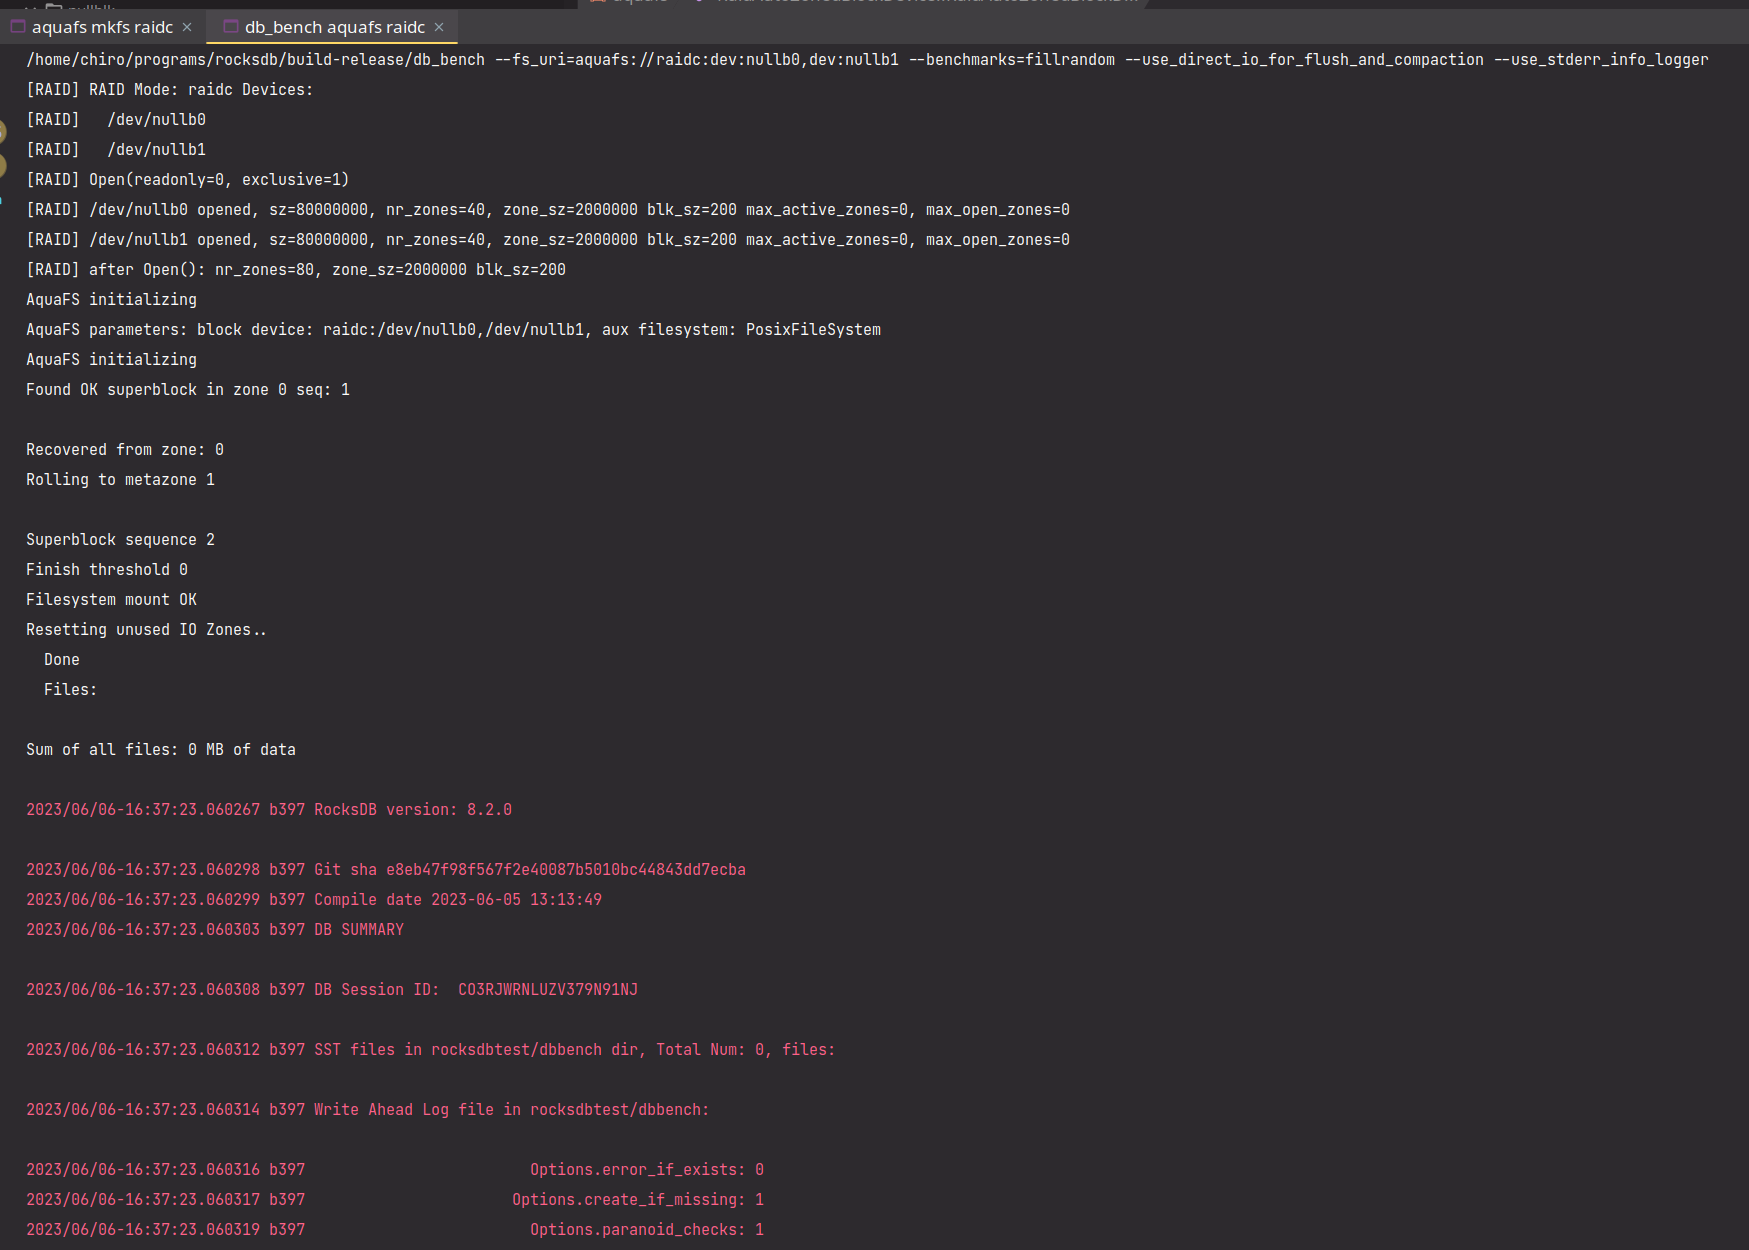
\includegraphics[width=0.85\textwidth]{fig/raid-data-check1}
  \caption{ 数据完整性测试1 }
  \label{check-data1}
\end{figure}

\begin{figure}[htbp]
  \centering
  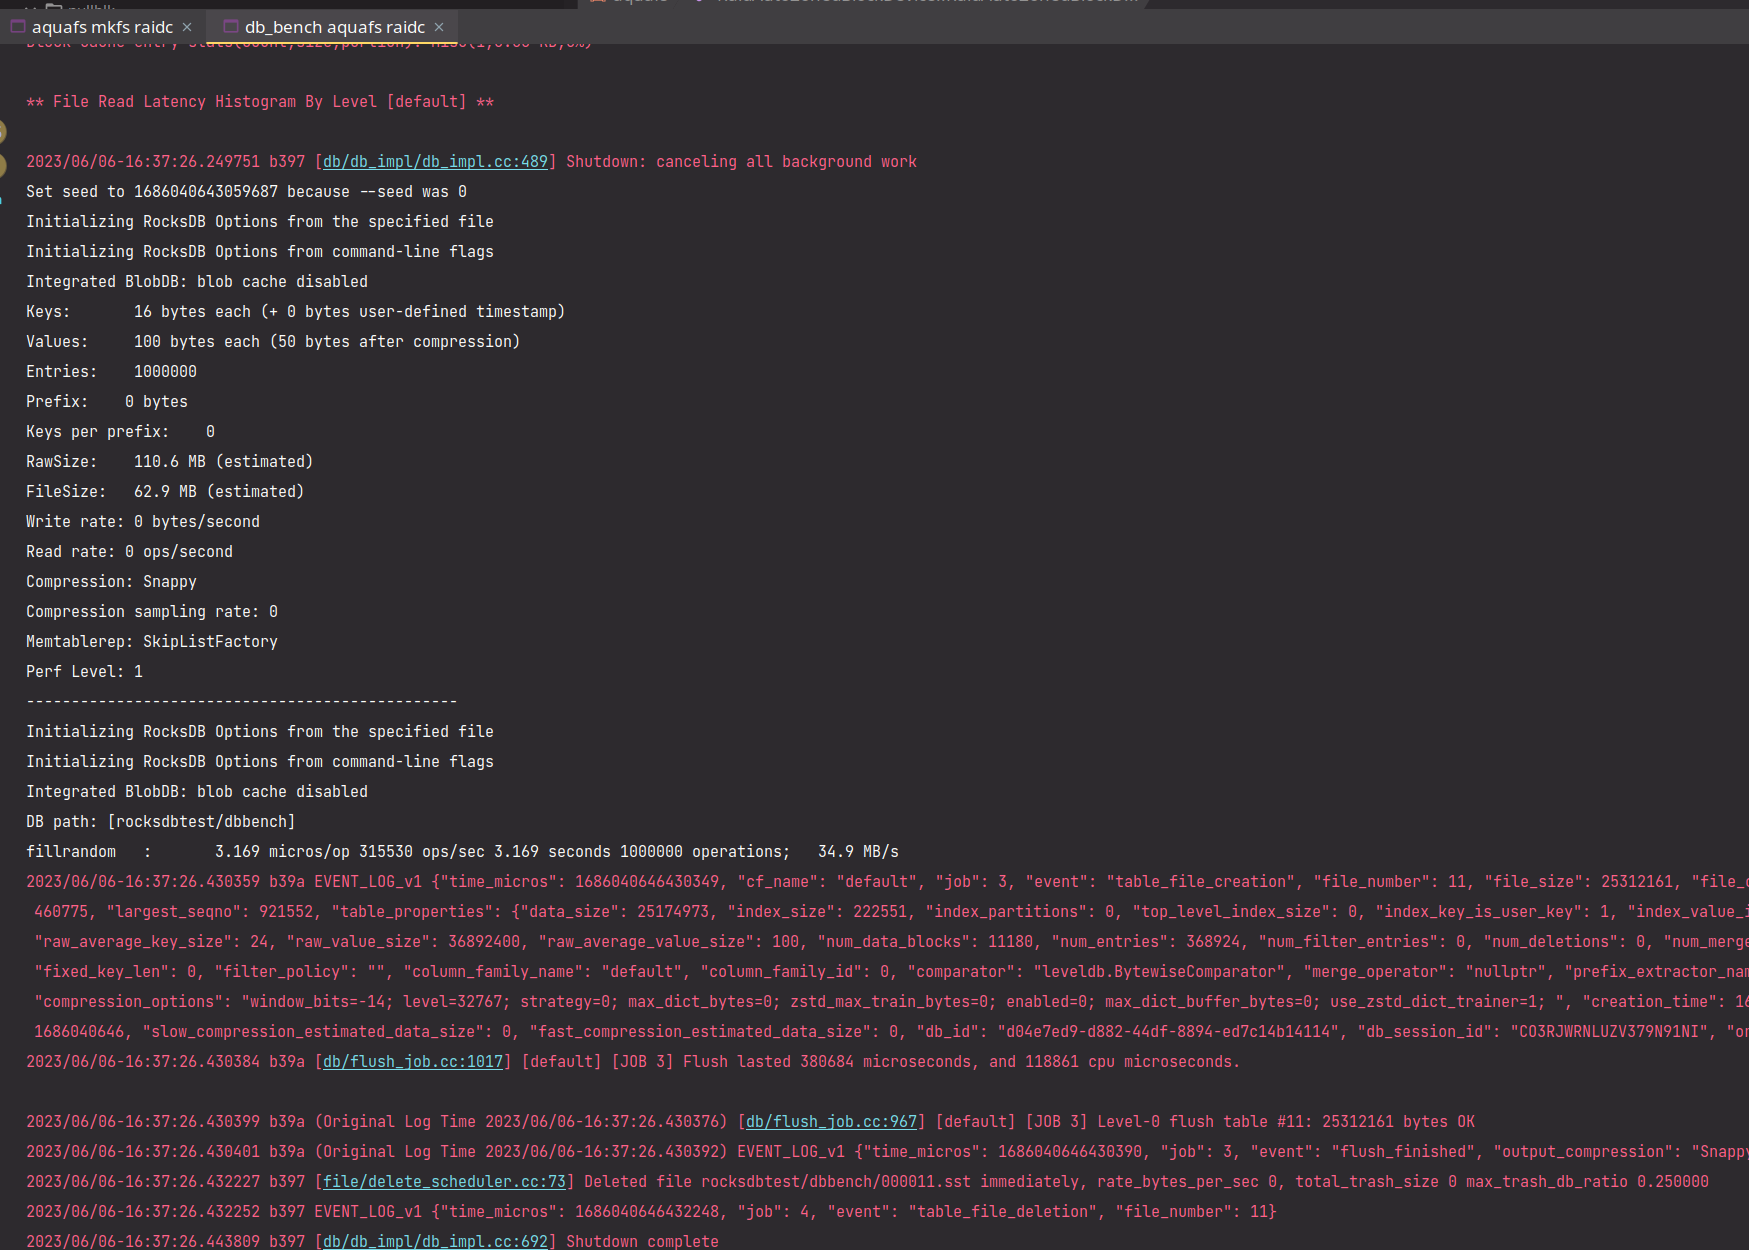
\includegraphics[width=0.85\textwidth]{fig/raid-data-check2}
  \caption{ 数据完整性测试2 }
  \label{check-data2}
\end{figure}

\begin{figure}[htbp]
  \centering
  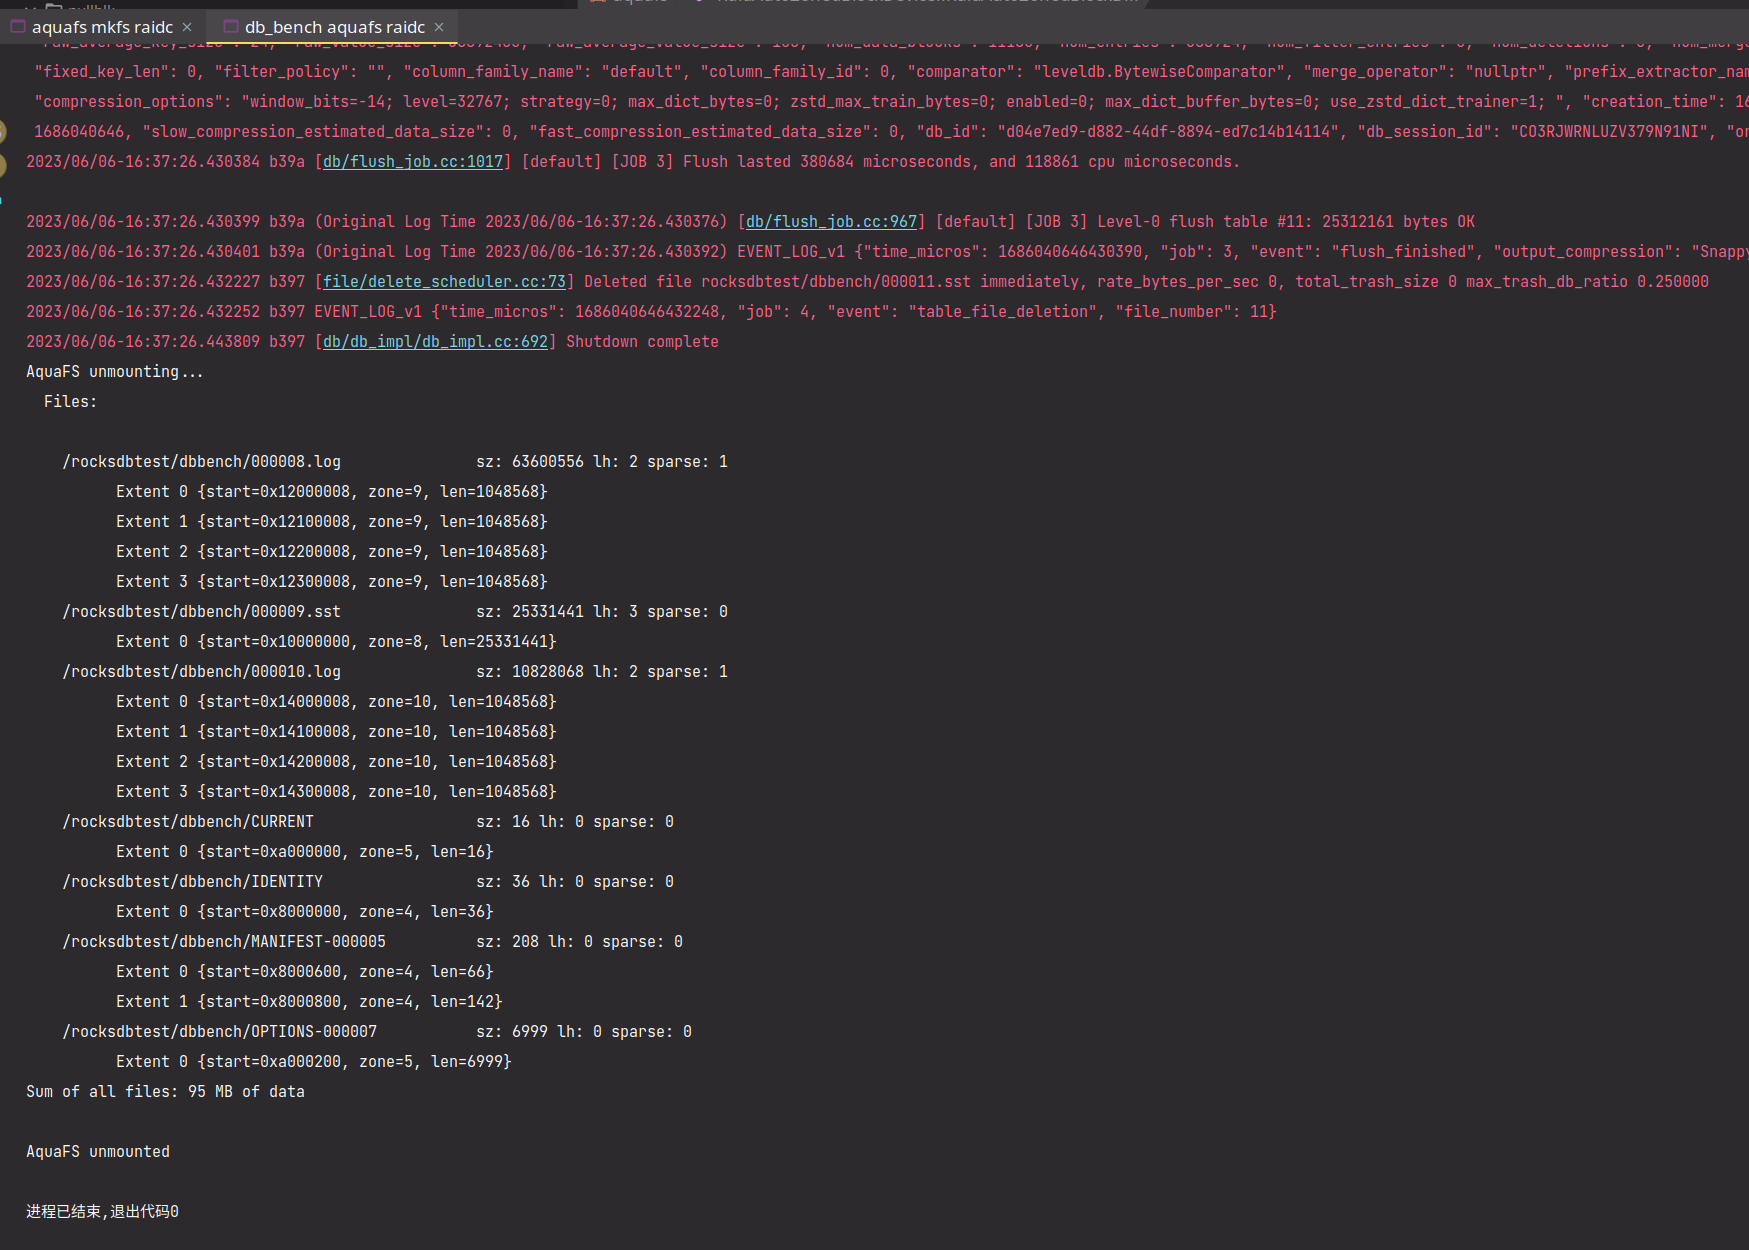
\includegraphics[width=0.85\textwidth]{fig/raid-data-check3}
  \caption{ 数据完整性测试3 }
  \label{check-data3}
\end{figure}

\subsubsection{使用 RAID 0 加速文件读写}

由于 ZenFS 并不支持 POSIX 规范的文件系统访问接口,所以无法将其挂载到 Linux 的 VFS 上,因此无法使用 Linux 的文件系统测试工具来测试其性能。这里使用的测试逻辑,与 RocksDB 使用 AquaFS 文件系统插件类似,都是通过写程序调用 AquaFS 的 API 来测试性能。

使用如下逻辑测试文件读写性能,并比较 RAID 0 的性能加速:

\begin{enumerate}
  \item 生成测试参数,包括文件大小、设备数量、RAID逻辑、随机种子等
  \item 创建文件系统,设置RAID逻辑等
  \item 在内存中生成一个指定大小的随机内容文件
  \item 重复进行多次:
  \begin{enumerate}
    \item 通过 \verb|aquafs restore| 将这个文件写入 AquaFS 文件系统
    \item 通过 \verb|aquafs dump| 将文件从 AquaFS 文件系统读出
    \item 通过 \verb|std::hash| 和 \verb|md5sum| 比较读出的文件和原文件是否一致
  \end{enumerate}
  \item 计算平均耗时,得到读写平均时间
\end{enumerate}

对多组数据进行测试,结果输出如图 \ref{raid0-speedup} 所示:

\begin{figure}[htbp]
  \centering
  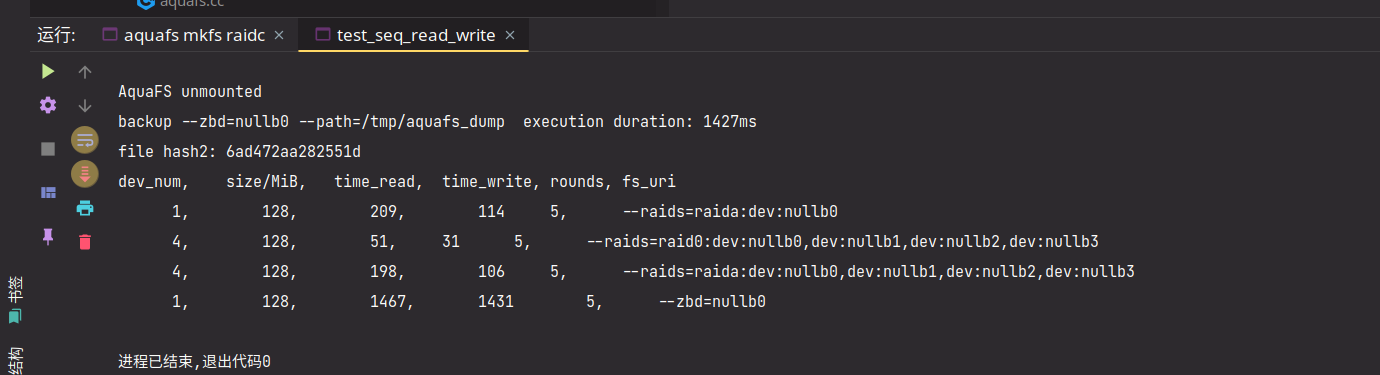
\includegraphics[width=0.85\textwidth]{fig/raid0-speedup}
  \caption{ RAID 0 加速测试 }
  \label{raid0-speedup}
\end{figure}

其得到的数据如表 \ref{raid0-speedup-table} 所示:

\begin{table}[htbp]
  \centering
  \caption{RAID 0 加速测试}
  \label{raid0-speedup-table}
  \begin{tabular}{cccccc}
    \hline
    \textbf{设备数量} & \textbf{文件大小(MiB)} & \textbf{平均读时间(ms)} & \textbf{平均写时间(ms)} & \textbf{次数} & \textbf{说明} \\
    \hline
    1 & 128 & 209 & 114 & 5 & 单盘分区 RAID \\
    4 & 128 & 51 & 31 & 5 &  多盘全盘 RAID 0 \\
    4 & 128 & 198 & 106 & 5 &  多盘分区 RAID \\
    1 & 128 & 1467 & 1431 & 5 &  ZenFS 默认 \\
    \hline
  \end{tabular}
\end{table}

可以看到,在单盘分区 RAID 的情况下,读写性能都有至少 N 倍的性能提升,而在多盘全盘 RAID 0 的情况下,读写性能有更大提升。

相比与 ZenFS 的默认读写,单盘分区读写由于使用 io\_uring、协程、重新构造读写请求等方式,性能有成倍的提升。具体提升幅度被能同时读写的 Zone 数量限制;而原版 ZenFS 只能单线程进行数据请求,因此性能较低。

相比与单设备的分区 RAID,多盘分区 RAID 有更大的性能提升。多盘意味着系统并行度更大,因此获得了更高的瞬时吞吐量。

而多盘全盘 RAID 0,由于采用的读写加速方式与分区 RAID 一致,其逻辑更加精简,因此性能更高。

\subsubsection{文件系统数据恢复测试}

测试逻辑:

\begin{enumerate}
  \item 生成随机大文件
  \item 使用 \verb|aquafs restore| 将文件写入 AquaFS 文件系统
  \item 在软件层面触发模拟硬件故障,使得一个 Dev Zone 下线
  \item 使用 \verb|aquafs dump| 将文件从 AquaFS 文件系统读出,观察是否能够正常读出
  \item 校验读出的文件和原文件是否一致
\end{enumerate}

使用 128 MiB 文件大小进行测试,测试过程如图 \ref{test-recovery} 所示。
在测试中,AquaFS 成功地检测到了 Zone 的故障,并且成功地从其他 Zone 中恢复了数据,维护了文件系统的数据完整性。

\begin{figure}[htbp]
  \centering
  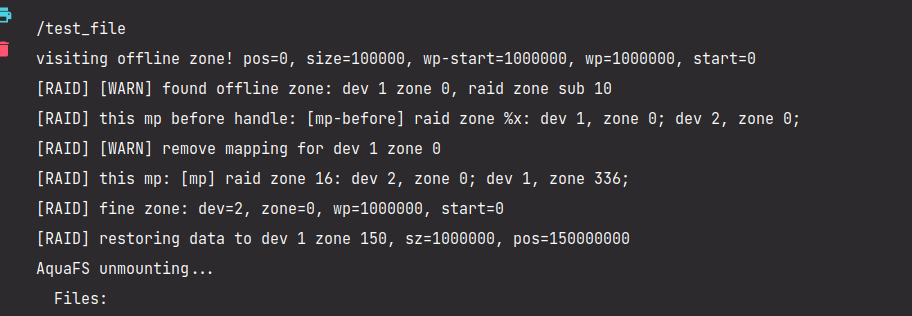
\includegraphics[width=0.85\textwidth]{fig/test-recovery}
  \caption{ 数据恢复测试 }
  \label{test-recovery}
\end{figure}

\subsubsection{文件系统性能测试}

由于可以使用内存作为存储后端,我们可以很便利地分析 AquaFS 的性能瓶颈,从而快速优化其性能。

我们使用 Linux \verb|perf| 工具进行性能分析,其中部分分析过程如图 \ref{test-perf} 所示。

\begin{figure}[htbp]
  \centering
  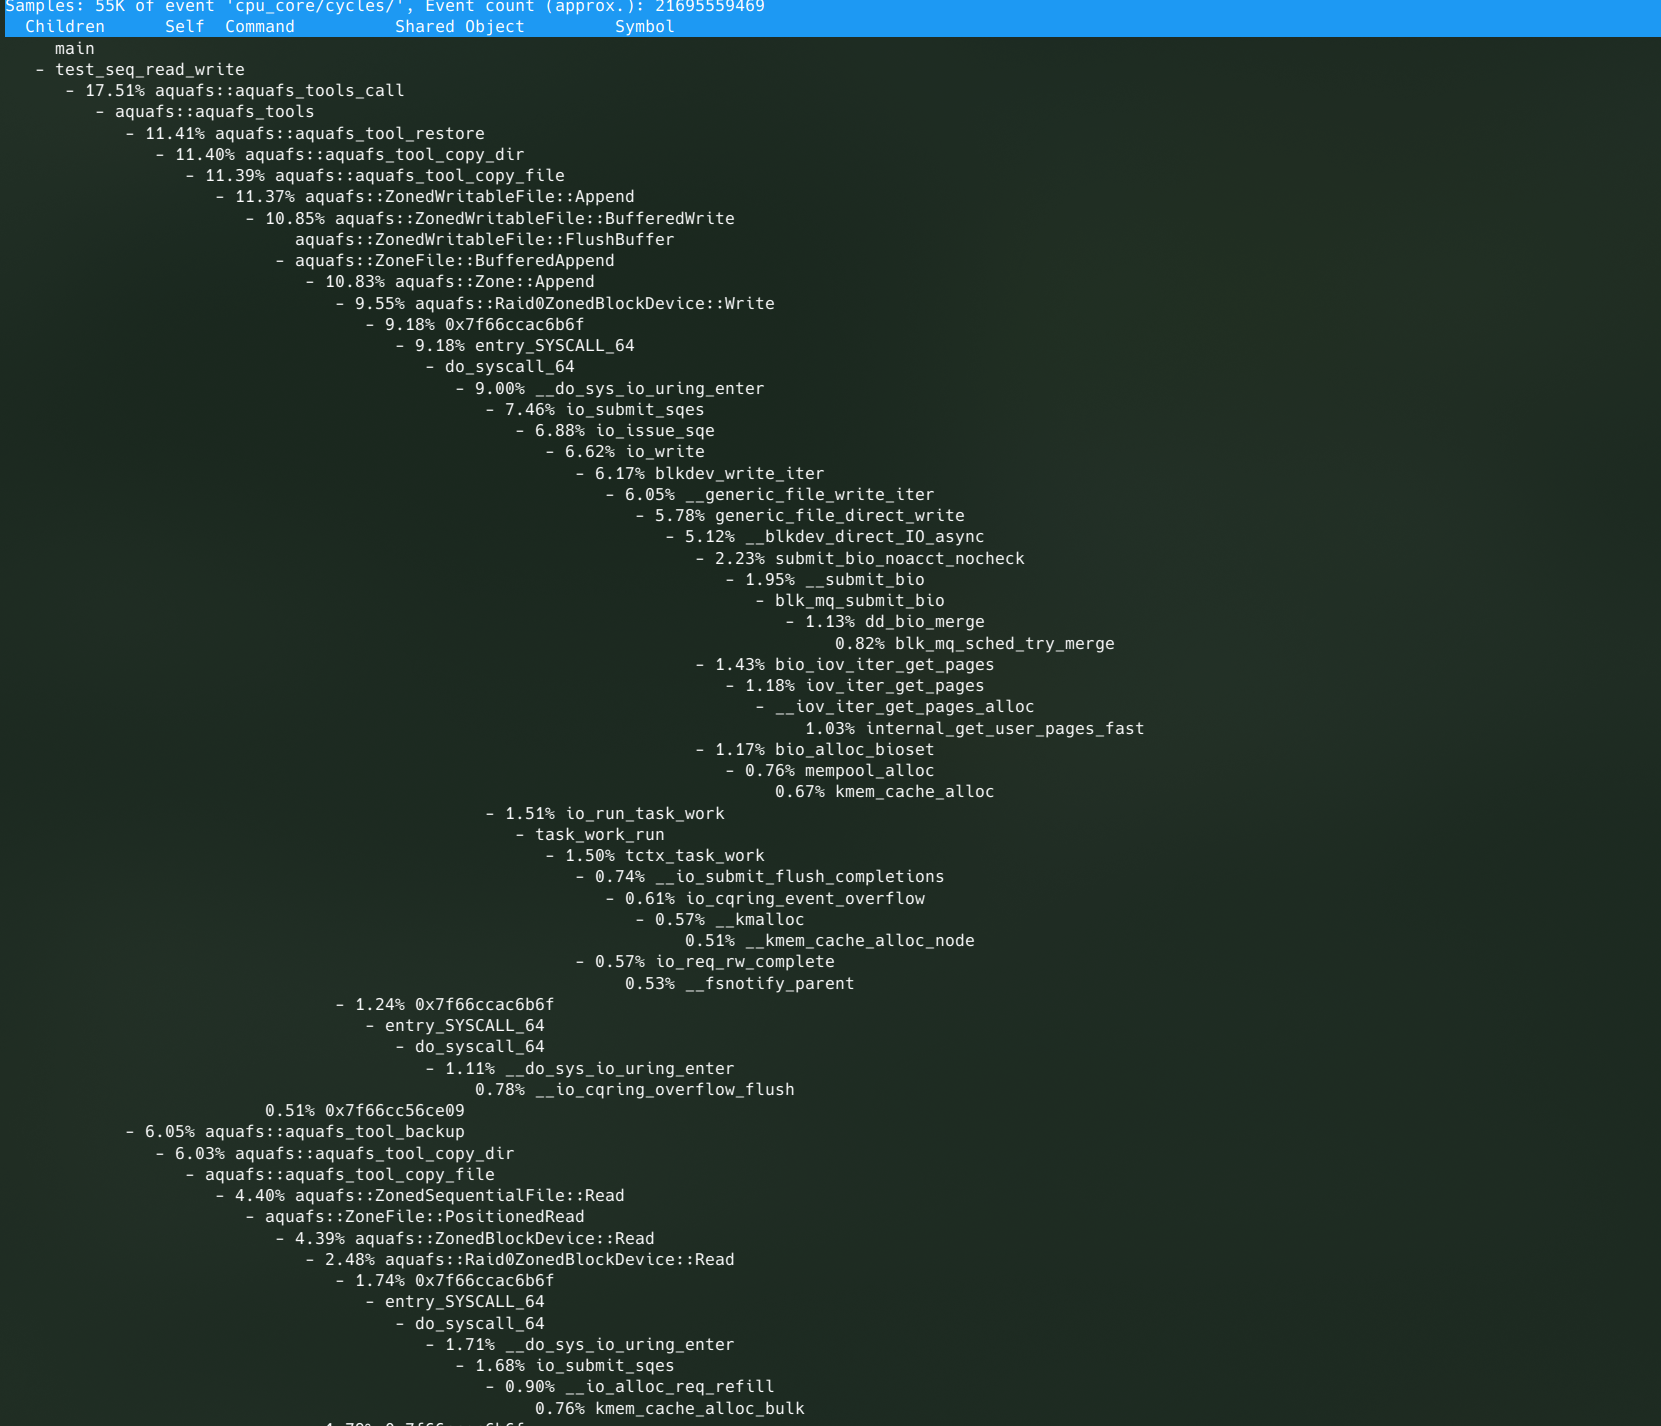
\includegraphics[width=0.85\textwidth]{fig/test-perf}
  \caption{ perf 性能分析 }
  \label{test-perf}
\end{figure}

可以看到,AquaFS 的性能瓶颈主要在于:

\begin{enumerate}
  \item \verb|entry_SYSCALL_64|:当前仍然使用内核态的 \verb|open|、\verb|read|、\verb|write| 等系统调用,导致系统频繁地从用户态切换到内核态,导致性能瓶颈。
  \item \verb|io_submit_sqes|:正在使用 io\_uring 的软件层面实现,可能使用方法还有可以优化的地方,造成 io\_uring 中一部分数据的锁争用。
\end{enumerate}

\subsubsection{ExtFS 功能和性能测试}

为了测试我们 ExtFS 的功能正确性,我们使用了本校操作系统实验课程中的测试脚本,对 ExtFS 进行了完整的功能测试,测试结果如下所示:

\begin{lstlisting}[language=bash]
  $ ./test.sh
  开始mount, mkdir, touch, ls, read&write, cp, umount测试测试脚本工程根目录: /home/chiro/os/fuse-ext2/fs/rfs/rfs/tests
  测试用例: /home/chiro/os/fuse-ext2/fs/rfs/rfs/tests/stages/mount.sh
  测试用例: /home/chiro/os/fuse-ext2/fs/rfs/rfs/tests/stages/mkdir.sh
  测试用例: /home/chiro/os/fuse-ext2/fs/rfs/rfs/tests/stages/touch.sh
  测试用例: /home/chiro/os/fuse-ext2/fs/rfs/rfs/tests/stages/ls.sh
  测试用例: /home/chiro/os/fuse-ext2/fs/rfs/rfs/tests/stages/remount.sh
  测试用例: /home/chiro/os/fuse-ext2/fs/rfs/rfs/tests/stages/rw.sh
  测试用例: /home/chiro/os/fuse-ext2/fs/rfs/rfs/tests/stages/cp.sh
  ============================================================================================================================    Finished dev [unoptimized + debuginfo] target(s) in 0.05s
       Running `/home/chiro/os/fuse-ext2/fs/rfs/rfs/target/debug/rfs --device=/home/chiro/ddriver -q /home/chiro/os/fuse-ext2/fs/rfs/rfs/tests/mnt`
  pass: case 1 - mount
  ============================================================================================================================pass: case 2.1 - mkdir /home/chiro/os/fuse-ext2/fs/rfs/rfs/tests/mnt/dir0
  pass: case 2.2 - mkdir /home/chiro/os/fuse-ext2/fs/rfs/rfs/tests/mnt/dir0/dir0
  pass: case 2.3 - mkdir /home/chiro/os/fuse-ext2/fs/rfs/rfs/tests/mnt/dir0/dir0/dir0
  pass: case 2.4 - mkdir /home/chiro/os/fuse-ext2/fs/rfs/rfs/tests/mnt/dir1
  ============================================================================================================================pass: case 3.1 - touch /home/chiro/os/fuse-ext2/fs/rfs/rfs/tests/mnt/file0
  pass: case 3.2 - touch /home/chiro/os/fuse-ext2/fs/rfs/rfs/tests/mnt/file1
  pass: case 3.3 - touch /home/chiro/os/fuse-ext2/fs/rfs/rfs/tests/mnt/dir0/file1
  pass: case 3.4 - touch /home/chiro/os/fuse-ext2/fs/rfs/rfs/tests/mnt/dir0/file2
  pass: case 3.5 - touch /home/chiro/os/fuse-ext2/fs/rfs/rfs/tests/mnt/dir1/file3
  ============================================================================================================================pass: case 4.1 - ls /home/chiro/os/fuse-ext2/fs/rfs/rfs/tests/mnt/
  pass: case 4.2 - ls /home/chiro/os/fuse-ext2/fs/rfs/rfs/tests/mnt/dir0
  pass: case 4.3 - ls /home/chiro/os/fuse-ext2/fs/rfs/rfs/tests/mnt/dir0/dir1
  pass: case 4.4 - ls /home/chiro/os/fuse-ext2/fs/rfs/rfs/tests/mnt/dir0/dir1/dir2
  ============================================================================================================================    Finished dev [unoptimized + debuginfo] target(s) in 0.05s
       Running `/home/chiro/os/fuse-ext2/fs/rfs/rfs/target/debug/rfs --device=/home/chiro/ddriver -q /home/chiro/os/fuse-ext2/fs/rfs/rfs/tests/mnt`
  pass: case 5.1 - umount /home/chiro/os/fuse-ext2/fs/rfs/rfs/tests/mnt
  pass: case 5.2 - check bitmap
  ============================================================================================================================    Finished dev [unoptimized + debuginfo] target(s) in 0.06s
       Running `/home/chiro/os/fuse-ext2/fs/rfs/rfs/target/debug/rfs --device=/home/chiro/ddriver -q /home/chiro/os/fuse-ext2/fs/rfs/rfs/tests/mnt`
  pass: case 6.1 - write /home/chiro/os/fuse-ext2/fs/rfs/rfs/tests/mnt/file0
  pass: case 6.2 - read /home/chiro/os/fuse-ext2/fs/rfs/rfs/tests/mnt/file0
  ============================================================================================================================pass: case 7.1 - prepare content of /home/chiro/os/fuse-ext2/fs/rfs/rfs/tests/mnt/file9
  pass: case 7.2 - copy /home/chiro/os/fuse-ext2/fs/rfs/rfs/tests/mnt/file9 to /home/chiro/os/fuse-ext2/fs/rfs/rfs/tests/mnt/file10
  ============================================================================================================================ 
  Score: 34/34
  pass: 通过所有测试 (34/34)
\end{lstlisting}

接着使用 \verb|dd| 工具,在本机的普通 1TiB SSD 上进行了简单的单文件读写测试:

\begin{lstlisting}[language=bash]
$ dd if=/dev/random of=mnt/random bs=1MiB count=64
输入了 64+0 块记录输出了 64+0 块记录67108864 字节 (67 MB, 64 MiB) 已复制,5.88972 s,11.4 MB/s
$ dd of=/dev/null if=mnt/random bs=1MiB count=64
输入了 64+0 块记录输出了 64+0 块记录67108864 字节 (67 MB, 64 MiB) 已复制,0.635838 s,106 MB/s
\end{lstlisting}

使用实验中的脚本进行读写性能测试,其测试逻辑为对文件中的某一固定的块反复读写:

\begin{lstlisting}
// 关闭模拟磁盘延迟,并且打开了缓存
Test loop: 1000000, Cache Blks: 512
  Finished release [optimized] target(s) in 0.05s
   Running `target/release/rfs --format -q -c --cache_size 512 /home/chiro/mnt`
Time: 30815.510034561157ms BW: 253.52492920733374MB/s
// 关闭模拟磁盘延迟,并且关闭了缓存
Test loop: 100000, Cache Blks: 0
  Finished release [optimized] target(s) in 0.05s
   Running `target/release/rfs --format -q /home/chiro/mnt`
Time: 8691.662073135376ms BW: 89.88499477156695MB/s
// 打开了模拟磁盘延迟,并且关闭了缓存
Test loop: 1000000, Cache Blks: 512
  Finished release [optimized] target(s) in 0.06s
   Running `target/release/rfs --format -q --latency -c --cache_size 512 /home/chiro/mnt`
Time: 30927.71863937378ms BW: 252.6051174707074MB/s
// 打开了模拟磁盘延迟,并且关闭了缓存
Test loop: 100, Cache Blks: 0
  Finished release [optimized] target(s) in 0.05s
   Running `target/release/rfs --format -q --latency /home/chiro/mnt`
Time: 9035.56513786316ms BW: 0.08646387780728894MB/s
\end{lstlisting}

可以看到,关闭缓存后,读写性能相比有缓存的大幅下降;而开启缓存后,读写性能相比无缓存的大幅提升。ExtFS 上的缓存工作正常且非常有效。在关闭了手动管理的缓存后,由于 Linux 本身为块设备提供了缓存,因此在不模拟磁盘延迟时关闭了手动管理的缓存,读写性能并没有下降太多。

由于 ExtFS 完成度还不高,所以 ExtFS 暂时还不是本项目的重点,后续会继续完善 ExtFS 的功能。

\subsection{AquaTurnner 智能调参模块测试}

首先进行warm\_up得到一组参数和目标指标值的csv文件如图 \ref{test-turnner1} 所示,现在由于只调整AquaFS参数,参数空间较小,主要包括垃圾回收的gc相关参数,块大小以及zone的大小参数等,后续考虑在融合文件系统后加入inode相关参数。

\begin{figure}[htbp]
  \centering
  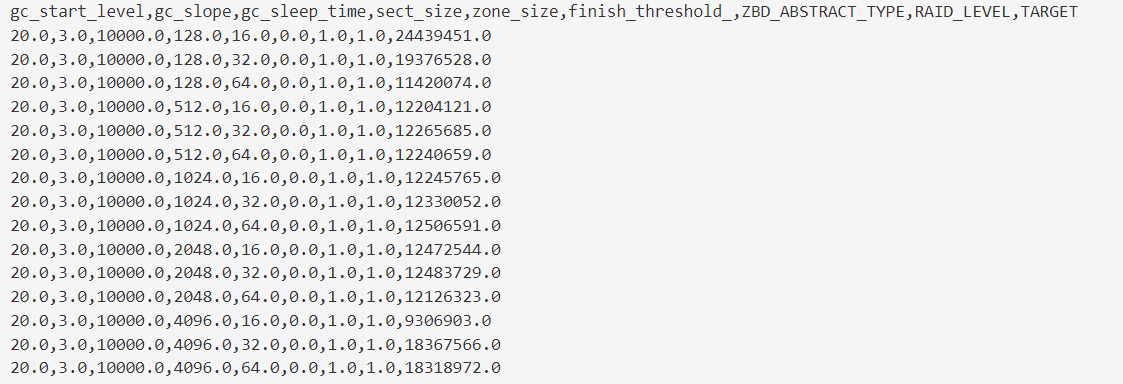
\includegraphics[width=0.85\textwidth]{fig/turnner1}
  \caption{ 调参测试数据 }
  \label{test-turnner1}
\end{figure}

设定参数进行AquaTuner的参数推荐流程,离散参数直接指定:

\begin{lstlisting}
SECT_SIZE_PARAM = 128
ZONE_SIZE_PARAM = 64
\end{lstlisting}

连续参数可以直接通过脚本defconfig获取。

接下来利用db\_bench进行参数跑分以及收集参数和目标值:

\begin{lstlisting}
  pre_throughput = 0
  now_throughput = 0
  for _ in range(1):
      sect_size = SECT_SIZE_PARAM
      zone_size = ZONE_SIZE_PARAM
      total_throughput = []
      for i in range(2):
          create_null_blk(sect_size, zone_size, 0, 64)
          os.system(CREATE_TMP_FILE)
          throughput_list = execute_adjust_param(2, sect_size, zone_size)
          total_throughput = total_throughput + throughput_list
          print("throughput list : {}".format(total_throughput))
          remove_null_blk()
      print("sect_size:{}".format(sect_size))
      print("zone_size:{}".format(zone_size))
      pre_throughput = now_throughput
      now_throughput = np.average(total_throughput)
\end{lstlisting}

代码的整体流程是,首先创建zone块,再在zone块上创建文件,得到跑分的吞吐量以及推荐参数,再将块zone块删除。

创建文件系统如下图所示,创建AquaFS的数据模块nullb0和作为log等文件存储的模块/tmp/aquafs。

\begin{lstlisting}
  CREATE_TMP_FILE = "mkdir -p /tmp/aquafs ;\
  sudo ../build/plugin/aquafs/aquafs mkfs --zbd nullb0 --aux-path /tmp/aquafs"
\end{lstlisting}

之后用db\_bench进行跑分,并进行智能调参模块的逻辑,按照指定推荐的离散参数跑一遍智能调参模块的结果如图 \ref{test-turnner2} 所示。

\begin{figure}[htbp]
  \centering
  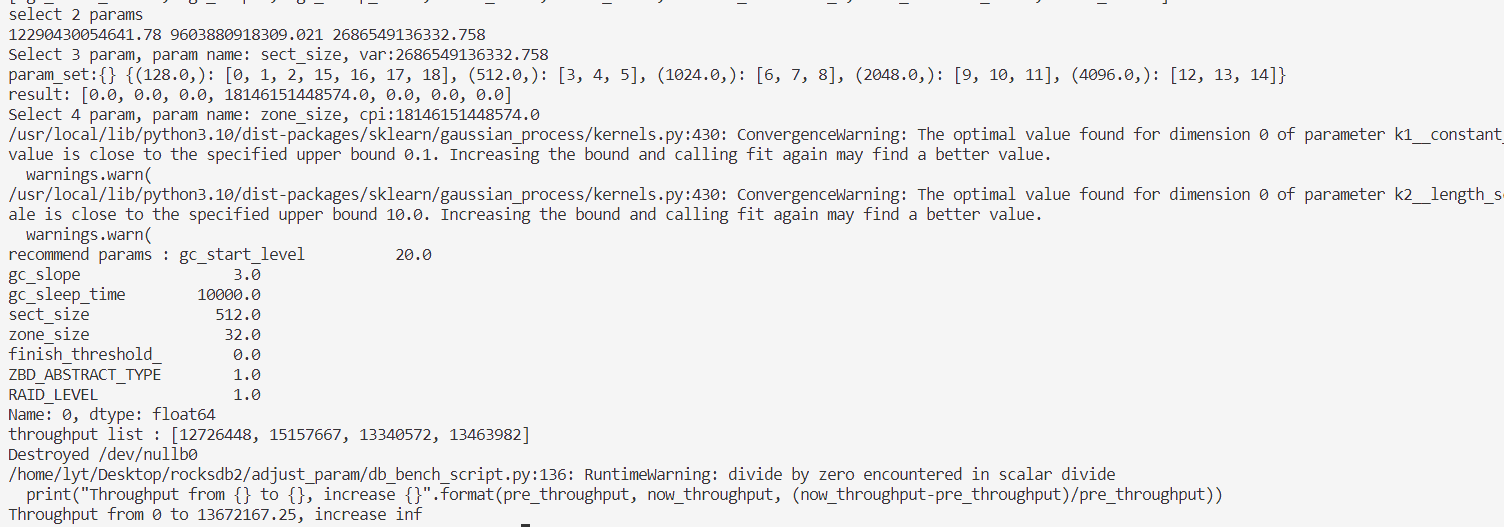
\includegraphics[width=0.85\textwidth]{fig/turnner2}
  \caption{ 调参测试过程 }
  \label{test-turnner2}
\end{figure}

在上图中推荐了两个参数,最重要的参数是sect\_size,其次是zone\_size,这符合现阶段的测试预期,因为我们的垃圾回收也就是gc还没有进行触发,,所以能够更改的参数现阶段只有块大小和zone\_size,而调参模块也根据现阶段的数据仓库中最优的参数进行了配置推荐。记录这里的平均吞吐量是13672167.25。

采用接下来的配置再进行测试:

\begin{lstlisting}
SECT_SIZE_PARAM = 512
ZONE_SIZE_PARAM = 32
\end{lstlisting}

最终结果如图 \ref{test-turnner3} 所示。

\begin{figure}[htbp]
  \centering
  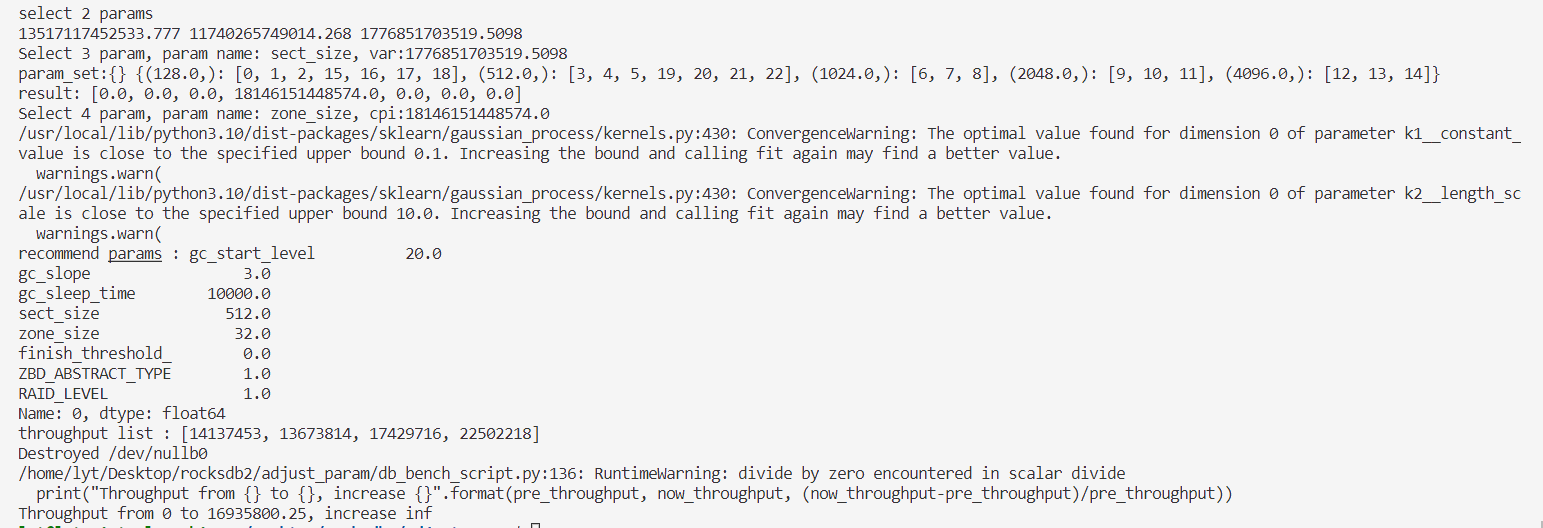
\includegraphics[width=0.85\textwidth]{fig/turnner3}
  \caption{ 调参测试结果 }
  \label{test-turnner3}
\end{figure}

平均吞吐量是16935800.25。相比于上一次的配置参数,吞吐量提升了23.87\%。

将不同轮次的调参结果进行对比如图 \ref{test-turnner} 所示,系统能够根据系统运行数据调整文件系统参数,从而逐步提高数据吞吐量。

\begin{figure}[htbp]
  \centering
  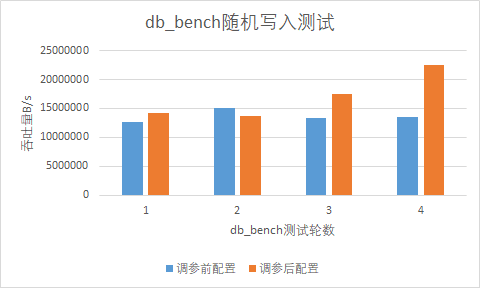
\includegraphics[width=0.85\textwidth]{fig/test-turnner}
  \caption{ 调参测试结果对比 }
  \label{test-turnner}
\end{figure}

后续还将尝试测试触发gc来测试gc的参数,以及尝试融合文件系统后对整体的inode以及其他参数进行自动调整。

